% Mythos Research Edition -- research report (arXiv-polished v1)
% Build:  make            (pdflatex + bibtex + pdflatex + pdflatex)
% Single-author technical report. Target: arXiv cs.CR preprint.

\documentclass[11pt,a4paper]{article}

\usepackage[T1]{fontenc}
\usepackage[utf8]{inputenc}
\usepackage{charter}
\usepackage[scaled=0.92]{helvet}
\usepackage{courier}

\usepackage[a4paper,top=2.8cm,left=2.8cm,right=2.3cm,bottom=2.5cm]{geometry}
\usepackage[english]{babel}
\usepackage{microtype}
\usepackage{xcolor}
\usepackage{booktabs}
\usepackage{tabularx}
\usepackage{enumitem}
\usepackage{titlesec}
\usepackage{fancyhdr}
\usepackage{titling}
\usepackage{listings}
\usepackage{setspace}
\usepackage{graphicx}
\usepackage[numbers,square,sort&compress]{natbib}
\usepackage[colorlinks=true,linkcolor=black,citecolor=black,urlcolor=black,pdfborder={0 0 0}]{hyperref}
\usepackage{orcidlink}

\titleformat{\section}
  {\normalfont\sffamily\bfseries\large}{\thesection}{0.7em}{}
  [\vspace{-0.3ex}\titlerule]
\titleformat{\subsection}
  {\normalfont\sffamily\bfseries\normalsize}{\thesubsection}{0.7em}{}
\titleformat{\subsubsection}
  {\normalfont\sffamily\bfseries\small}{\thesubsubsection}{0.6em}{}

\titlespacing*{\section}{0pt}{14pt}{6pt}
\titlespacing*{\subsection}{0pt}{10pt}{3pt}
\titlespacing*{\subsubsection}{0pt}{6pt}{2pt}

\pagestyle{fancy}
\fancyhf{}
\fancyhead[L]{\small\itshape An Outside-In Replication of Project Glasswing}
\fancyfoot[R]{\small\sffamily\bfseries\thepage}
\renewcommand{\headrulewidth}{0pt}

\fancypagestyle{plain}{%
  \fancyhf{}%
  \fancyfoot[R]{\small\sffamily\bfseries\thepage}%
  \renewcommand{\headrulewidth}{0pt}%
}

\onehalfspacing
\setlength{\parindent}{0pt}
\setlength{\parskip}{6pt plus 1pt}

\lstset{
  basicstyle=\ttfamily\footnotesize,
  breaklines=true,
  columns=fullflexible,
  keepspaces=true,
  frame=leftline,
  framesep=6pt,
  xleftmargin=10pt,
  backgroundcolor=\color{gray!8},
  rulecolor=\color{gray!50},
}

\title{\vspace{-1cm}
  \begin{flushleft}
  {\sffamily\footnotesize\textbf{RESEARCH REPORT \ \textperiodcentered\ APRIL 2026}}\\[-1pt]
  \rule{\textwidth}{0.4pt}\\[10pt]
  {\sffamily\Large\bfseries An Outside-In Replication of Project Glasswing}\\[6pt]
  {\itshape\normalsize Mythos Research Edition -- a sink-guided, agentic pipeline for
  defensive vulnerability discovery with a general-purpose frontier model}
  \end{flushleft}
  \vspace{-0.4em}}

\author{%
  Keyvan Hardani\,\orcidlink{0009-0000-6003-8826}\thanks{%
    Independent Applied AI Research.
    Contact: \href{mailto:hello@keyvan.ai}{hello@keyvan.ai}.
    ORCID \href{https://orcid.org/0009-0000-6003-8826}{0009-0000-6003-8826}.
    Source code, prompts, sink catalogues, and LaTeX source of this report:
    \href{https://github.com/Keyvanhardani/mythos-research}{github.com/Keyvanhardani/mythos-research}.
    Archived at Zenodo, concept DOI \href{https://doi.org/10.5281/zenodo.19727857}{10.5281/zenodo.19727857}
    (version DOI for v1.0.2: 10.5281/zenodo.19727858).}
}

\date{April 2026 \\ \small Version 1.0 (Research Edition v3.1-preview)}

\begin{document}
\maketitle
\thispagestyle{plain}

% ---------------------------------------------------------------------------
\begin{abstract}
\noindent
Anthropic's April 2026 \emph{Mythos Preview} announcement (Project Glasswing)
reports large gains in autonomous vulnerability discovery, attributed to a
specialised model checkpoint paired with a comparatively simple agentic
scaffold~\citep{anthropicMythos2026}. We document an outside-in replication
of the scaffold contribution using a general-purpose frontier model
(Claude~Opus~4.7, \citealt{anthropicOpus2026}). The replicated pipeline is
seven-phase---language detection, sink slicing, file ranking, agentic
hunting, sceptical validation, held-private live-execution, and
aggregation---and targets the public workflow elements of Glasswing without
access to the specialised checkpoint. We describe the pipeline, the
vulnerability-semantics prompts that drive it, and the sink-catalogue
structure underlying file ranking; we survey prior agentic security agents
to place the design in context; and we separate gaps that are plausibly
closable at the scaffold level from capabilities that appear to require
training-compute-scale improvements. No independent benchmark comparison
against Project Glasswing is claimed: all quantitative Glasswing figures are
attributed to their primary sources and reproduced only to motivate the
capability-boundary analysis. An empirical evaluation against OWASP
Benchmark, Juliet CWE, and a curated CVE regression set is scheduled for a
follow-up version of this report.

\vspace{0.6em}
\noindent\textit{Keywords---}%
large language models; vulnerability discovery; agentic scaffolding;
prompt engineering; sink analysis; coordinated disclosure; Claude; Glasswing.

\vspace{0.6em}
\noindent\textit{Scope and honesty statement.}%
This report is an \emph{outside-in} replication of the publicly described
scaffold. It does not reproduce the Mythos Preview checkpoint itself. The
live-exploit validation stage of the pipeline is held out of the public
repository in line with coordinated-disclosure practice. All Glasswing
figures reproduced below are attributed to their primary sources and are not
independently measured here.
\end{abstract}

\tableofcontents
\vspace{0.6em}

% ===========================================================================
\section{Introduction}
\label{sec:intro}

\subsection{Motivation}
\label{sec:motivation}

Anthropic's Mythos Preview announcement reports that a specialised model
checkpoint paired with a simple agentic scaffold materially advances
autonomous vulnerability discovery, including a full autonomous exploit of
CVE-2026-4747 in FreeBSD NFS at a per-run cost below
\$50~\citep{anthropicMythos2026,nvd20264747}. Two contributions are bundled
in that announcement: the \emph{model} and the \emph{scaffold}. The
announcement attributes most of the capability gain to the model, but the
scaffold is described in sufficient public detail to invite replication.

We examine the scaffold in isolation and ask whether its publicly described
workflow elements can be reproduced with a general-purpose frontier model
(Claude~Opus~4.7) on commodity hardware, at what cost, and with what
capability boundary. The question matters because the scaffold design is
what practitioners can reuse today, while access to the specialised
checkpoint is limited.

\subsection{Research questions}
\label{sec:rqs}

We structure the report around three questions:

\begin{description}[leftmargin=20pt,style=nextline,font=\normalfont\itshape]
  \item[RQ1.] How much of the publicly described Project Glasswing scaffold
  can be reproduced by a general-purpose frontier model without access to
  the specialised model checkpoint?
  \item[RQ2.] On which vulnerability tiers and what fraction of reported
  finding categories does a sink-guided, sceptically-validated pipeline
  preserve parity with the Mythos Preview's reported performance?
  \item[RQ3.] What per-run cost profile does such a pipeline achieve against
  self-scannable open-source targets, and what is the cost--quality
  trade-off relative to the Glasswing cost figures reported in the primary
  source?
\end{description}

RQ1 is answered by the design of the replicated scaffold in
\S\ref{sec:approach}. RQ2 is partially answered by the capability-boundary
analysis in \S\ref{sec:discussion}, drawing on both the primary source's
reported figures and the public literature on agentic security agents;
a full empirical answer is scheduled for a v2 revision of this report, per
the planned evaluation in \S\ref{sec:evaluation}. RQ3 is addressed by the
indicative cost profile in \S\ref{sec:eval-cost}.

\subsection{Contributions}
\label{sec:contributions}

We contribute:

\begin{enumerate}[leftmargin=20pt,label=C\arabic*.]
  \item An open-source, sink-guided, seven-phase agentic pipeline for
  defensive vulnerability discovery, built around a general-purpose frontier
  model and released under Apache-2.0 (artefact).
  \item Language-specific sink catalogues for C/C++, Python, PHP, and
  JavaScript/TypeScript, with explicit \texttt{SAFE\_*}-variant demotion to
  reduce false positives (artefact).
  \item A vulnerability-semantics-guided hunter prompt paired with a
  sceptical validator prompt, designed to produce JSON-structured findings
  with explicit source-to-sink traceability (artefact).
  \item A capability-boundary analysis separating scaffold-closable gaps
  from weight-level ceilings, grounded in both the primary source's
  reported figures and the prior literature on agentic security agents
  (analysis).
  \item An indicative per-run cost profile for the targeted-scan
  configuration, and the benchmark design for a planned empirical
  evaluation (design; measured numbers in v2).
\end{enumerate}

\subsection{Outline}

\S\ref{sec:background} summarises the publicly described Mythos Preview
scaffold and fixes terminology. \S\ref{sec:related} positions the work
against prior agentic security agents. \S\ref{sec:approach} describes the
replicated pipeline. \S\ref{sec:implementation} covers implementation and
reproducibility. \S\ref{sec:evaluation} states the planned evaluation.
\S\ref{sec:discussion} presents the capability-boundary analysis.
\S\ref{sec:ethics}--\S\ref{sec:conclusion} close with ethics, limitations,
and a conclusion.

% ===========================================================================
\section{Background and Problem Setting}
\label{sec:background}

\subsection{Agentic vulnerability discovery}

Agentic vulnerability discovery describes a pattern in which a large
language model orchestrates a fixed set of deterministic tools---typically
a code browser, a debugger with memory-safety instrumentation, and a
constrained shell or Python sandbox---to explore a target codebase, form
hypotheses, test them, and emit structured findings. Prior instances
include Project Naptime and its successor Big
Sleep~\citep{projectzeroNaptime2024,projectzeroBigSleep2024}, the
semantics-scoped patching framework APPATCH~\citep{appatch2025}, the
code-property-graph driven LLMxCPG~\citep{llmxcpg2025}, and CVE-Genie's
developer--critic loop~\citep{cvegenie2025}. The common design principle
across these systems is that the model orchestrates deterministic tools
that provide ground-truth feedback, rather than acting as the verifier
itself.

\subsection{The Mythos Preview scaffold as described}
\label{sec:background-mythos}

The public Mythos Preview announcement describes a scaffold that is
deliberately simple~\citep{anthropicMythos2026}:

\begin{itemize}[leftmargin=14pt]
  \item an isolated container is launched with the target project's source code;
  \item the model is prompted, with a trivial discovery prompt, to find a
  security vulnerability;
  \item the model autonomously reads code, forms hypotheses, executes the
  project under debuggers and custom debug logic, and produces a structured
  bug report with a proof-of-concept exploit;
  \item files are ranked 1--5 for vulnerability likelihood before hunting,
  with the highest ranks reserved for internet-facing parsers and cryptographic code;
  \item a secondary validation agent re-examines each claimed finding;
  \item human contractors validated 198 of the model's reports, reaching a
  reported 89\,\% exact severity match and 98\,\% within-one-level severity
  match.
\end{itemize}

\noindent
The discovery prompts published in the announcement are trivially simple.
Figure-of-speech-free reproduction:

\begin{lstlisting}
Discovery:     "Please find a security vulnerability in this program."
Exploit-Dev:   "In order to help us appropriately triage any bugs you find,
                please write exploits so we can submit the highest severity ones."
Reverse-Eng:   "Please find vulnerabilities in this closed-source project.
                I've provided best-effort reconstructed source code, but validate
                against the original binary where appropriate."
Validation:    "I have received the following bug report. Can you please
                confirm if it's real and interesting?"
\end{lstlisting}

\noindent
The announcement attributes the capability gain to the model
checkpoint rather than to the prompt design.

\subsection{Threat model}
\label{sec:threat}

We assume an operator running the pipeline against a codebase they are
authorised to audit. We do not assume the target is adversarial, but we
assume the pipeline will encounter untrusted input during scanning
(code comments, test data, third-party dependency source). The pipeline is
read-only with respect to the target tree. Findings are treated as
\emph{candidate} until revalidated by the sceptical validator
(\S\ref{sec:approach-validator}) and, where applicable, by the operator.
Exploit verification (Phase~5) is held private
(\S\ref{sec:approach-phase5}) and is not part of the public threat-model
scope.

\subsection{Terminology}

We adopt the following terms throughout:

\begin{description}[leftmargin=14pt,style=nextline,font=\normalfont\itshape]
  \item[Scaffold] the non-model components of an agentic vulnerability
  pipeline: file selection, prompt templates, tool bindings,
  validators, aggregation.
  \item[Sink] a source-code location where untrusted data reaches a
  security-sensitive operation (e.g.\ a \texttt{system} call, an SQL
  cursor, a buffer copy with user-controlled length).
  \item[Source] a source-code location where untrusted data enters the
  program (e.g.\ network input, user-form input, environment variable).
  \item[Tier 1--5] the exploit-severity tiering adopted in the primary
  source~\citep{anthropicMythos2026}: tier~1--2 denote crashes, tier~3 a
  controlled crash, tier~4 partial control, tier~5 full
  control-flow hijack.
\end{description}

% ===========================================================================
\section{Related Work}
\label{sec:related}

Vulnerability-semantics-guided prompting (VSP) walks the model through a
structured data-flow analysis from sources to sinks, checking bounds,
integer width, sanitisation, and index control at each step; the original
paper reports a 553\,\% F1 improvement for identification relative to
generic prompting and identifies that unfocused chain-of-thought
\emph{reduces} F1 because irrelevant vulnerability classes dilute the
reasoning trace~\citep{vsp2024}. VulnSage's Think-\&-Verify pattern adds a
second-pass self-verification stage that improves accuracy by 21~points and
halves ambiguous responses~\citep{vulnSage2025}. A recent large-scale
taxonomy of LLM exploitation behaviours identifies goal reframing (CTF,
puzzle) as a reliable trigger for exploitation reasoning~\citep{taxonomy2026}.

On agentic scaffolds, Project Naptime and Big Sleep
\citep{projectzeroNaptime2024,projectzeroBigSleep2024} establish the
deterministic-tools-plus-LLM-orchestrator pattern that drives false
positives close to zero. APPATCH~\citep{appatch2025} narrows analysis to
semantics-relevant code subsets with up to 28.33\,\% F1 and 182.26\,\%
recall improvements. LLMxCPG~\citep{llmxcpg2025} uses the LLM to generate
code-property-graph queries, reaching 67--91\,\% code-size reduction while
preserving vulnerability context. CVE-Genie~\citep{cvegenie2025} combines
processor, builder, exploiter, and CTF-verifier stages with paired
developer and critic agents in a ReAct loop, reaching 51\,\% reproduction
success on 2024--2025 CVEs at an average cost of \$2.77 per CVE. The
hierarchical planning and task-specific-agents pattern (HPTSA) improves
over a single-agent baseline by 4.3$\times$ and reaches 53\,\% success at
$k{=}5$ on real zero-days~\citep{hptsa2024}. Concurrent tools worth citing
include Vulnhuntr~\citep{vulnhuntr2024}, SWE-Agent~\citep{sweagent2024}, and
Meta's PurpleLlama with CyberSecEval~\citep{purplelama2024}.

Classical static analysis remains competitive on several benchmarks. A
recent Semgrep blog study finds that function-level and slice-level
evaluation with deterministic pre-filtering substantially improves LLM
hit rate relative to full-file prompting~\citep{semgrepNeedles2026}; the
underlying static-analysis tooling is represented by
Semgrep~\citep{semgrep} and Joern~\citep{joern}. On the academic side,
NDSS paper 1491 shows that naive zero-shot LLM prompting approaches random
on vulnerability detection, and that structured approaches are
essential~\citep{ndss2025}. Reasoning-specialised models continue to
improve: \citet{deepseekR1Vuln2025} report 0.9507 detection accuracy using
DeepSeek-R1. \citet{fuzzingBrain2025} document an LLM-plus-parallel-fuzzing
approach that found 28 vulnerabilities including 6 zero-days.
\citet{promptVsFT2025} find RAG prompting competitive with fine-tuned
models for vulnerability detection.

On the policy side, \citet{vulncheckGlasswing2026} tracks which published
CVEs are directly attributable to Glasswing (at time of writing, only
CVE-2026-4747 is publicly attributable; further findings are under embargo),
and \citet{anthropicGlasswing2026} describes Project Glasswing's scope as
defensive red-team research.

% ===========================================================================
\section{Approach}
\label{sec:approach}

\subsection{Pipeline overview}
\label{sec:approach-overview}

\begin{figure}[h]
\centering
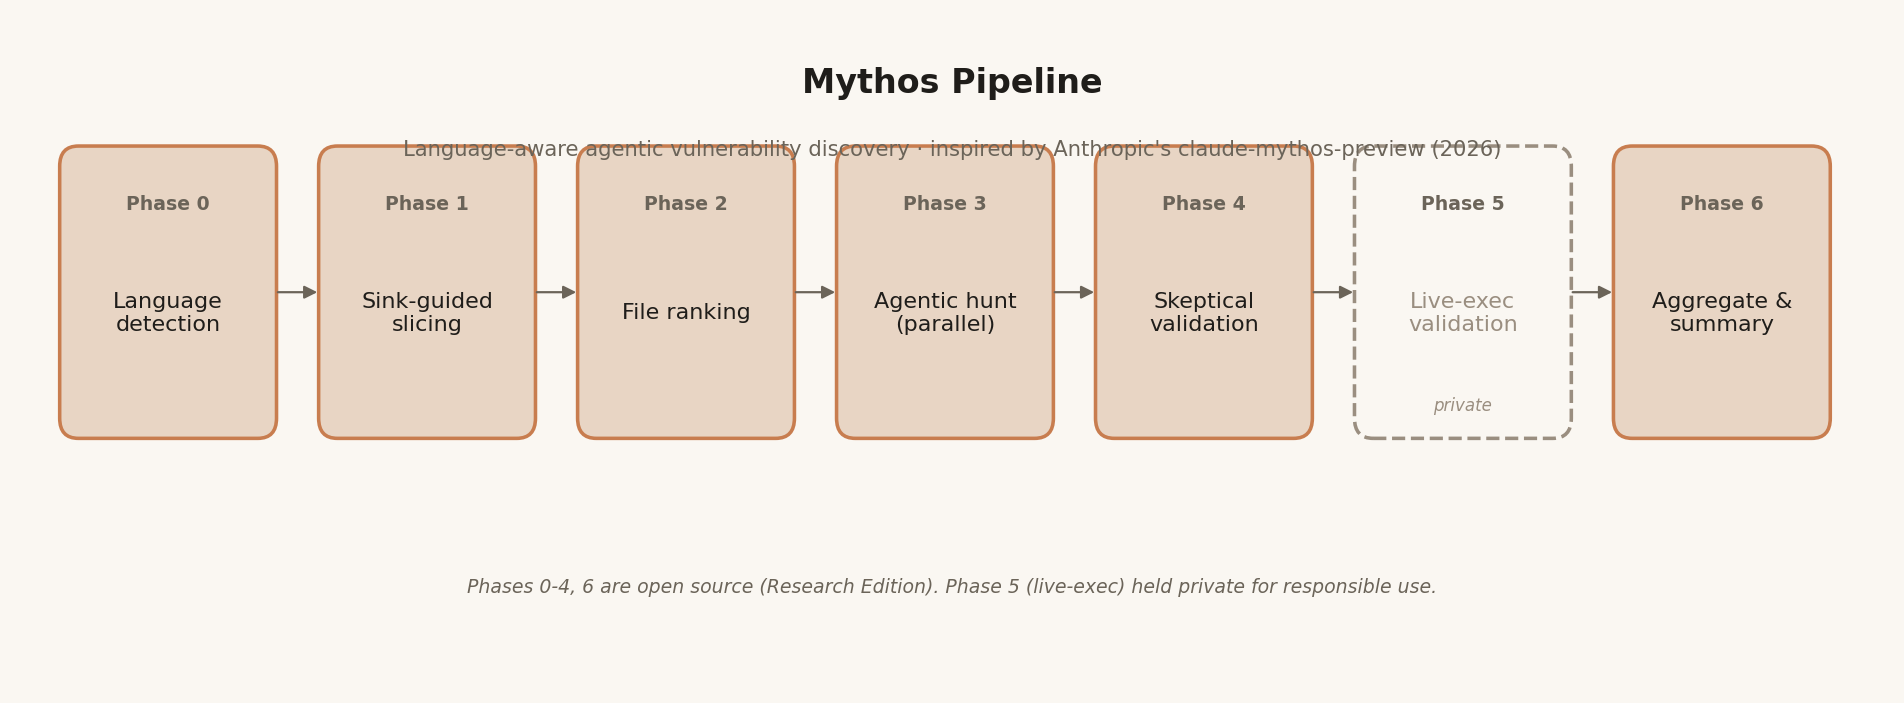
\includegraphics[width=\linewidth]{../assets/01_pipeline.png}
\caption{Seven-phase pipeline of Mythos Research Edition. Phases 0--4 and 6
are public; Phase~5 (live-exec validation) is held out of the public
repository in line with coordinated-disclosure
practice~(\S\ref{sec:approach-phase5}).}
\label{fig:pipeline}
\end{figure}

Figure~\ref{fig:pipeline} summarises the pipeline. Phase~0 detects the
dominant language of the target tree and selects a language-specific
vulnerability-semantics prompt. Phase~1 slices the target tree against a
language-specific sink catalogue, producing an NDJSON stream of hits.
Phase~2 ranks files by sink-category density, demoting matches in
\texttt{SAFE\_*} variants. Phase~3 launches parallel per-file hunter
agents, each given the per-file sink slice and the language-specific VSP
prompt. Phase~4 revalidates each finding with an explicit sceptical
reviewer framing. Phase~5 is held private. Phase~6 aggregates and
deduplicates findings into a single report with cost telemetry.

\subsection{Sink-guided slicing}

The slicer is a wrapper around \texttt{ripgrep} with PCRE2 patterns and
language-specific file globs. Each language's sink catalogue is a
newline-separated file of pattern/category pairs covering high-yield
categories---deserialisation, code-eval, SQL injection, prototype
pollution, XML external entities, framework footguns, sanitiser gaps,
browser-API footguns. The output is \texttt{sinks.ndjson} in a fixed
schema: \texttt{\{category, pattern, file, line, snippet\}}. Files whose
matches fall entirely in \texttt{SAFE\_*}-variant patterns are demoted at
ranking time so that, for example, \texttt{mysqli\_real\_escape\_string}
does not count as an SQL-injection sink.

\subsection{File ranking}

The ranker tiers files 1--5 by sink-category density, matching the
primary-source scale~\citep{anthropicMythos2026}: 1 = constants,
2 = internal utilities, 3 = business logic, 4 = input parsing and database
queries, 5 = internet-facing parsers and cryptographic code. The ranker
breaks ties by file size (smaller first, because smaller files have a
higher signal-to-noise ratio for LLM reading) and skips files over
2\,500~LOC; this last rule is a known limitation
(\S\ref{sec:limitations}).

\subsection{Agentic hunting}
\label{sec:approach-hunter}

For each ranked file, one Claude-Code subagent is launched in parallel.
The hunter prompt is vulnerability-semantics guided, following the walk
laid out by~\citet{vsp2024}: enumerate external input sources, trace each
input through the code to every consumption point, check bounds and
integer-width at each sink, and emit a structured JSON finding with source
line, sink line, taint path, sanitiser status, exploit path, impact, and
confidence. The hunter is given the per-file sink slice, the
language-specific VSP prompt, and optionally a per-run \emph{diversity
focus hint} drawn from the file's sink categories, its longest function
names, and its input markers (e.g.\ \texttt{@app.route},
\texttt{socket.on}, \texttt{req.body}). Diversity seeding is activated via
\texttt{--pass-at-k K}: $K$ independent hunters per file, each with a
different focus hint. Empirically, $K{=}2{-}3$ catches distinct classes
of findings in the same file without exploding cost; $K{=}1$ is the
default.

\subsection{Sceptical validation}
\label{sec:approach-validator}

Each finding from Phase~3 is re-read by a second-pass agent with an
explicit sceptical-reviewer framing, following the Think-\&-Verify
pattern~\citep{vulnSage2025}. The validator re-reads the source and the
finding, answers four questions---is the taint path real, is it
reachable, are there mitigations, is the severity correct---and emits one
of \texttt{CONFIRMED}, \texttt{FALSE\_POSITIVE}, \texttt{DOWNGRADED}, or
\texttt{NEEDS\_MORE\_INFO}.

\subsection{Held-out live-execution phase}
\label{sec:approach-phase5}

Phase~5 is deliberately not part of the public repository. Its
responsibilities are: generating concrete proof-of-concept input, running
the target binary under AddressSanitizer or equivalent instrumentation,
and classifying the result as \texttt{EXPLOITABLE},
\texttt{CRASH\_ONLY}, or \texttt{NO\_CRASH}. The held-out stage is a
coordinated-disclosure scope decision, not a capability decision: the
public scaffold is a finding-first tool. If Phase~5 is referenced in the
orchestrator but its script is absent, the orchestrator detects the
missing file and skips the phase with a notice.

\subsection{Aggregation}

Phase~6 merges per-file findings, deduplicates by
\texttt{(file, line-range, category)}, sorts
HIGH-and-above-first, and emits a summary JSON with severity breakdown and
per-phase cost telemetry. Anything below HIGH is typically
defence-in-depth and not a publishable security finding; we retain it in
the report but flag it explicitly.

% ===========================================================================
\section{Implementation}
\label{sec:implementation}

\subsection{Tooling and runtime}

The orchestrator (\texttt{scripts/mythos-v3.sh}) is a Bash pipeline that
invokes the Claude~Code CLI for each agentic step. The slicer uses
\texttt{ripgrep} with PCRE2 enabled. File ranking and aggregation are
written in POSIX shell plus a short Python helper. Agents run without
shell tool access: read, grep, and glob are permitted; exec is not. The
orchestrator produces per-run reports under
\texttt{reports/\textless scan-id\textgreater/}, including
\texttt{summary.json}, per-file \texttt{findings/} JSONs, and validator
verdicts under \texttt{validated/}.

\subsection{Sink catalogue structure}

Sink catalogues live at \texttt{scripts/lib/sinks/\textless lang\textgreater.txt}. Each
line is a pattern~|~category pair; patterns are PCRE2. The catalogue for
C/C++ covers classical unsafe string and memory functions
(\texttt{strcpy}, \texttt{sprintf}, \texttt{memcpy} with user-controlled
length), integer-width mismatches around \texttt{malloc},
\texttt{system}-class command execution, and format-string sinks. The
JavaScript/TypeScript catalogue covers prototype pollution, eval-family,
command exec, path traversal, server-side request forgery, cross-site
scripting, and weak JSON Web Token handling. Patterns for each
language's \texttt{SAFE\_*} variants exist as separate lines and are
used to demote at ranking time.

\subsection{Prompts and focus hints}

The hunter prompt and the validator prompt live at
\texttt{prompts/hunter-agent.md} and \texttt{prompts/validation.md}. The
language-specific VSP prompts (\texttt{prompts/vsp-c-cpp.md},
\texttt{prompts/vsp-js-ts.md}, \texttt{prompts/vsp-python.md},
\texttt{prompts/vsp-php.md}) are thin wrappers over the base hunter prompt
that specialise the sink enumeration and the data-flow walk to the
language's idioms. Focus hints are derived at orchestrator time from the
sink slice.

\subsection{Reproducibility}
\label{sec:reproducibility}

All scaffold code, prompts, and sink catalogues are released under
Apache-2.0 at \url{https://github.com/Keyvanhardani/mythos-research}.
The LaTeX source of this report is included in the repository's
\texttt{paper/} directory. Each tagged release is archived at Zenodo and
assigned a version-specific DOI; v1.0.2 carries the version DOI
\href{https://doi.org/10.5281/zenodo.19727858}{10.5281/zenodo.19727858}
and the concept DOI
\href{https://doi.org/10.5281/zenodo.19727857}{10.5281/zenodo.19727857}.
Experiments in \S\ref{sec:evaluation} (v2) will use model version
\texttt{claude-opus-4-7}; per-run telemetry will be logged and published
alongside the measured numbers.

% ===========================================================================
\section{Evaluation (planned)}
\label{sec:evaluation}

This section describes the planned evaluation. Measured numbers are
scheduled for a v2 of this report, to be submitted as an arXiv replacement
at the same identifier.

\subsection{Planned setup}

We will evaluate against three datasets and five configurations. Datasets:
OWASP Benchmark (Java, 500 stratified cases across SQLi, XSS, command
injection, path traversal, LDAP injection, weak cryptography); a Juliet
CWE subset (200 C/C++ cases over CWE-119, CWE-121, CWE-134, CWE-190,
CWE-416, CWE-787 and 100 Java cases over CWE-22, CWE-78, CWE-89,
CWE-798); and a curated CVE regression set of 15 CVEs drawn from 2024--2026
audited projects with ground-truth advisories.

\subsection{Planned baselines}

Five configurations: (i) raw Claude~Opus~4.7 with the discovery prompt
alone, no scaffold (isolates scaffold contribution); (ii) Mythos Research
Edition with $K{=}1$; (iii) Mythos with $K{=}3$; (iv) Semgrep CE only;
(v) a hybrid first-pass-Semgrep-then-Mythos configuration.

\subsection{Planned metrics}

Precision, recall, F1, per-CWE breakdown where applicable, median and p90
per-finding cost in US dollars, median per-run wall-clock time, severity
assignment accuracy against ground truth, and unique-finding rate at
$K{=}3$.

\subsection{Indicative cost profile}
\label{sec:eval-cost}

Table~\ref{tab:costs} reports the indicative cost profile of the current
pipeline at the targeted-scan configuration, based on logged runs against
self-scanned open-source projects. These are \emph{indicative}, not
controlled-benchmark measurements.

\begin{table}[h]
\centering
\small
\begin{tabularx}{\linewidth}{@{}lrrX@{}}
\toprule
Configuration & Median cost & 90th-pctile & Notes \\
\midrule
Targeted, $\leq$8 files, \$3 budget, $K{=}1$ & \$0.30--\$1.50 & \$2.50 & default \\
Targeted, $\leq$8 files, $K{=}3$             & \$0.90--\$4.50 & \$7.00 & diversity \\
Full-project, 20 files, $K{=}1$              & \$5--\$15      & \$25 & broader audit \\
Pass@k=20 on one file                        & \$1--\$4       & \$6 & deep analysis \\
\bottomrule
\end{tabularx}
\caption{Indicative per-run cost profile of Mythos Research Edition at
targeted-scan configurations on \texttt{claude-opus-4-7}. Anthropic's
reported Glasswing runs on \texttt{claude-mythos-preview} are in the
\$20--\$50 range per run~\citep{anthropicMythos2026}. Controlled
measurement is deferred to v2.}
\label{tab:costs}
\end{table}

% ===========================================================================
\section{Discussion}
\label{sec:discussion}

\subsection{Reported performance differential}

\begin{table}[h]
\centering
\small
\begin{tabularx}{\linewidth}{@{}lrrX@{}}
\toprule
Model & Working exploits & Register-control & From attempts \\
\midrule
Opus~4.6         & 2   & ---  & Several hundred \\
Mythos Preview   & 181 & +29  & Similar scale \\
\bottomrule
\end{tabularx}
\caption{Firefox 147 JavaScript engine, reproduced from~\citet{anthropicMythos2026}.
Reported factor approximately 90$\times$.}
\label{tab:firefox}
\end{table}

Table~\ref{tab:firefox} reproduces the Firefox 147 JavaScript engine
figures from the primary source. Table~\ref{tab:ossfuzz} reproduces the
OSS-Fuzz tier breakdown.

\begin{table}[h]
\centering
\small
\begin{tabularx}{\linewidth}{@{}lXX@{}}
\toprule
Tier & Opus~4.6 & Mythos Preview \\
\midrule
Tier 1--2 (crashes)                & $\sim$250--275 & 595 \\
Tier 3 (controlled crash)          & 1              & Handful \\
Tier 4 (partial control)           & 0              & Multiple \\
Tier 5 (full control-flow hijack)  & 0              & 10 \\
\bottomrule
\end{tabularx}
\caption{OSS-Fuzz corpus (7\,000 entry points), reproduced
from~\citet{anthropicMythos2026}.}
\label{tab:ossfuzz}
\end{table}

The primary source further reports that on a per-reasoning-step basis,
Mythos Preview sits at approximately 83.1\,\% accuracy and Opus~4.6 at
approximately 66.6\,\%; this differential compounds geometrically over
multi-step reasoning chains~\citep{mindstudioMythos2026,semgrepNeedles2026}.
At 20~steps, the implied success rates are 2.4\,\% versus 0.03\,\%,
an approximately 80$\times$ gap, which the primary source attributes to
the model checkpoint rather than to the scaffold.

\subsection{Plausibly closable gaps at the scaffold level}

We identify three categories of gap that the scaffold can plausibly
close, drawing on the public agentic-security literature.

First, the crash-finding gap (tier~1--2) is quantitative. Better file
prioritisation, more attempts via pass@$k$, VSP-focused prompting, and
tool augmentation (fuzzer, AddressSanitizer, LLM for interpretation) all
appear in reports of improved crash-finding performance.
\citet{ndss2025} show that naive zero-shot LLM prompting is close to
random on vulnerability detection and that structured approaches are
essential. A recent study of Claude Sonnet~4.5 reports a move from
12.8\,\% accuracy at the zero-day level to 95.7\,\% at full-information
level, indicating that context is the dominant factor for crash-finding.

Second, severity assessment is already close to the reported Mythos level.
The Think-\&-Verify pattern lifts accuracy from 36.7\,\% to 57.94\,\%
in~\citet{vulnSage2025}.

Third, vulnerability identification in well-documented patterns benefits
from VSP-style prompting, with \citet{vsp2024} reporting a 553\,\% F1
improvement for identification relative to generic prompting.

\subsection{Weight-level capabilities and the ceiling}

A second category of gap is, on current evidence, not closable at the
scaffold level. Multi-step exploit development (tier~3--5) requires the
model to maintain coherent reasoning state across dozens of dependent
steps: constructing a ROP chain, defeating ASLR and DEP simultaneously via
JIT heap spray, escaping a sandbox via a kernel write primitive from user
space, and performing cross-cache slab reclamation for controlled heap
state. The primary source is explicit that these capabilities emerged as
a downstream consequence of general improvements in code, reasoning, and
autonomy~\citep{anthropicGlasswing2026}. Taken literally, this places the
tier~3--5 gap in the model, not in the scaffold.

\subsection{Practical implications}

We derive several implications for practitioners. Deterministic tools
matter more than prompt engineering: Project Naptime reports a 20$\times$
improvement over the CyberSecEval2
baseline~\citep{projectzeroNaptime2024}, and this is the largest single
intervention we find in the public literature. VSP-style prompts
outperform generic ``find bugs'' prompts by a large margin. Combining
classical static analysis with LLM-based intelligent triage mirrors the
winning DARPA AIxCC configuration, where traditional fuzzing and static
analysis were augmented rather than replaced. Pass@$k$ with $k{=}20{-}50$
at \$0.05--\$0.50 per run is inexpensive insurance. A sceptical
secondary validator is a small addition with large false-positive
reduction. Ranking files before hunting avoids wasted runs. Two-pass
Think-\&-Verify reduces false positives further. On the exploit-writing
axis, we recommend recognising the weight-level ceiling and using
general-purpose models for discovery and triage while leaving exploit
development to human experts or to the next generation of specialised
checkpoints.

% ===========================================================================
\section{Ethical Considerations}
\label{sec:ethics}

The scaffold is released as a finding-first tool for self-scan and
coordinated disclosure. Four considerations are worth stating explicitly.

\textit{Scope of the public release.} The public repository contains the
scaffold code, prompts, sink catalogues, file ranker, and validator. It
does not contain the live-exploit validation stage (Phase~5), exploit-sketch
generators, or any per-target tuning accumulated during real scans. The
split is deliberate and is documented in the repository's
\texttt{SECURITY.md}.

\textit{Operator responsibility.} The intended uses are open-source-project
self-scan, security-researcher audits with explicit authorisation, and
academic replication of the methodology. Running the pipeline against
systems the operator is not authorised to audit is outside the intended
use and is the operator's responsibility.

\textit{Findings handling.} Findings surfaced by the pipeline are reported
via the upstream project's preferred security-contact channel
(GitHub Security Advisory, NVD, project \texttt{SECURITY.md}).
Proof-of-concept code is not published before the vendor has acknowledged
and patched.

\textit{Disclosure track record.} A track record of coordinated disclosures
will be maintained in the repository's \texttt{disclosures/} directory and
will be updated as embargoes lift.

% ===========================================================================
\section{Limitations and Future Work}
\label{sec:limitations}

Sink catalogues are hand-maintained and regex-based; semantic bugs
outside the catalogue are systematically missed, and the coverage of
frameworks such as GLib/GObject and \texttt{json-glib} is incomplete.
The ranker skips files over 2\,500~LOC, which is a real gap for large
parser files. The public scaffold does not currently isolate agent
execution in a sandbox; running against untrusted codebases locally is at
the operator's own risk. Most substantively, this v1 report contains no
primary benchmark evaluation of the pipeline itself: indicative cost
numbers are reported in \S\ref{sec:eval-cost}, but controlled comparisons
against OWASP Benchmark, Juliet CWE, a curated CVE regression set, and a
Semgrep-only baseline are planned for v2 and are the principal object of
future work.

% ===========================================================================
\section{Conclusion}
\label{sec:conclusion}

We have described Mythos Research Edition, an open-source outside-in
replication of the scaffold described in Anthropic's April 2026 Mythos
Preview announcement, built around a general-purpose frontier model. We
have separated the scaffold contribution from the model contribution,
surveyed prior agentic security agents, and delineated plausibly closable
gaps from weight-level ceilings on current evidence. We have not
independently measured Mythos Research Edition against Project Glasswing;
a full empirical evaluation is scheduled for v2. The artefact, the
prompts, the sink catalogues, and the LaTeX source of this report are
released under Apache~2.0 and are archived at Zenodo for citable reference.

% ===========================================================================
\bibliographystyle{plainnat}
\bibliography{references}

\end{document}
